% Supplement generated from audited experiment reports; see local provenance manifest.
\clearpage
\nolinenumbers
\appendix
\setcounter{table}{0}
\renewcommand{\thetable}{S\arabic{table}}
\renewcommand{\theHtable}{supp.\arabic{table}}
\setcounter{figure}{0}
\renewcommand{\thefigure}{S\arabic{figure}}
\renewcommand{\theHfigure}{supp.\arabic{figure}}
\setcounter{equation}{0}
\renewcommand{\theequation}{S\arabic{equation}}
\renewcommand{\theHequation}{supp.\arabic{equation}}
\raggedbottom
\section*{Supplementary Material}
This supplement provides implementation and evaluation details, baseline configurations, and deployment results for EfficientGeo. The final student uses 128 teacher-subspace and 32 random-subspace targets with 256-pixel inputs. Retrieval results use the original encoder unless otherwise stated. Additional ablations and qualitative retrieval examples follow.

\section{Implementation and Evaluation Details}
\label{sec:supp-implementation}
\subsection{Method Implementation Details}
\paragraph{Foundation teacher.}
We adapt DINOv3 ViT-7B using bidirectional InfoNCE. With zero-based block indices, blocks 0--19 are frozen, blocks 20--35 use LoRA on attention QKV and output projections, and blocks 36--39 are fully fine-tuned. LoRA uses rank 8, scaling factor 16, and dropout 0.1.

\paragraph{Stage I.}
The intermediate teacher is initialized from pretrained DINOv3 ViT-B.

\paragraph{Stage II and optimization.}
The student is RepViT-M1.5, initialized with the official ImageNet-1K pretrained weights (450-epoch release). DG-SAM uses radius 0.1 in both distillation stages, with distillation-only perturbation and a full-objective second pass on the same augmented batch. Backbone computation uses BF16. Descriptor normalization, similarities, and distillation targets use FP32.

\subsection{Training and Optimization Settings}
We train the foundation teacher, intermediate teacher, and student on University-1652 for 10, 10, and 30 epochs, respectively. Each update uses 32 location pairs. The foundation teacher uses four GPUs with eight pairs per GPU. Stage I uses two GPUs with 16 pairs per GPU and cross-GPU feature gathering. Stage II uses one GPU with 32 pairs. The final student uses training seed~0.

\paragraph{Foundation teacher.}
The initial learning rate is $10^{-4}$ for LoRA and the logit scale, and $10^{-5}$ for fully fine-tuned backbone parameters. We use Adam with decoupled weight decay through DeepSpeedCPUAdam, with $(\beta_1,\beta_2)=(0.9,0.999)$ and $\epsilon=10^{-8}$. Weight decay is 0.01 for decayed parameters and zero for biases, normalization parameters, and the logit scale. The cosine schedule uses a 5\% warm-up. DeepSpeed ZeRO-2 offloads optimizer states to CPU, with BF16 computation and gradient clipping at 1.0. During the final four adaptation epochs, the teacher's University-1652 D$\rightarrow$S R@1 increases only from 96.73\% to 96.81\%, while S$\rightarrow$D R@1 is 97.29\% at both endpoints.

\paragraph{Stage I.}
DeepSpeedCPUAdam uses an initial learning rate of $10^{-4}$, weight decay 0.01, $(\beta_1,\beta_2)=(0.9,0.999)$, and $\epsilon=10^{-8}$, with cosine decay and a 5\% warm-up. TG-HND selects five different-location negatives independently in each retrieval direction, with loss weight 0.1. Auxiliary calibration has weight 0.05, and the two softmax fusion weights are initialized to 0.3 and 0.7.

\paragraph{Stage II.}
We optimize the student with AdamW at learning rate $10^{-4}$ and weight decay $10^{-4}$, excluding biases and normalization parameters from decay. Cosine decay follows a 0.1-epoch warm-up and ends at 1\% of the initial learning rate. The initial retrieval temperature is 0.07 and is learned during training. Label smoothing is 0.1. The ADSD weight increases linearly from zero to 0.2 over five epochs.

\subsection{Calibration and Subspaces}
\label{sec:supp-subspace}
\paragraph{Auxiliary calibration.}
\label{sec:supp-calibration}
For auxiliary calibration, foundation-teacher features at block indices 28 and 36 supervise the intermediate teacher's block-10 feature. The teacher and intermediate feature dimensions are 4096 and 768. Each calibration bridge separately projects the CLS token and attention-pooled patch feature, concatenates them, and applies an MLP with hidden width 2048.

\paragraph{Subspace construction and student mappings.}
For the images $\mathcal X_\ell^v$ of training location $\ell$ and view $v$, centroid construction and centering are defined by
\begin{equation}
\begin{aligned}
m_\ell^v&=\operatorname{norm}\!\left(\frac{1}{|\mathcal X_\ell^v|}
\sum_{x\in\mathcal X_\ell^v}z_M(x)\right),\\
\mu&=\frac{1}{2L}\sum_{\ell=1}^L\sum_{v\in\{u,s\}}m_\ell^v,
\end{aligned}
\label{eq:adsd_centroids}
\end{equation}
where $\mathcal X_\ell^v$ contains images of location $\ell$ in view $v$, $L$ is the number of training locations, and $\operatorname{norm}(a)=a/\|a\|_2$.

We extract descriptors without augmentation from the 701 University-1652 training locations, yielding 1,402 equally weighted centroids. The principal basis is obtained by FP64 singular-value decomposition of the centered centroids. The final student uses 128 principal directions and 32 random directions. The random basis is constructed by QR orthonormalization of a Gaussian matrix sampled using a random seed. It is not constrained to be orthogonal to the principal basis. Both bases and $\mu$ remain fixed during training.


The principal student mapping consists of a linear projection and a two-layer GELU residual MLP of hidden width 920. At initialization, its final layer is scaled once so that its output has the same root-mean-square magnitude as the linear output on a fixed calibration set of 768 training images. Its learnable multiplier starts at $10^{-3}$. The random mapping is linear. Predictions are normalized before cosine matching. Centering by $\mu$ is applied to the intermediate-teacher descriptors before projection. The student mappings directly predict the corresponding normalized targets. All mappings and projection assets are discarded at inference.

\subsection{Gradient-Balanced Weighting}
\label{sec:supp-balancing}
GBW adjusts the teacher-subspace and random-subspace weights according to the gradients they produce on the shared student descriptors. For each branch $b\in\{p,r\}$ and view $v\in\{u,s\}$, let $\mathcal L_b^v$ be the mean cosine loss and $Z_S^v$ the student descriptors. We compute the gradient norm for each view and average the two norms:
\begin{equation}
G_b=\tfrac12\!\sum_{v\in\{u,s\}}\left\|\nabla_{Z_S^v}\mathcal L_b^v\right\|_F.
\end{equation}
A scalar gate $\xi$ sets $w_p=0.5+\sigma(\xi)$ and $w_r=1.5-\sigma(\xi)$. The weights sum to two, each lies between 0.5 and 1.5, and both start at one when $\xi=0$. The gate is trained to bring the weighted gradient magnitudes $w_pG_p$ and $w_rG_r$ closer, by minimizing their squared log difference:
\begin{equation}
\begin{aligned}
\mathcal L_{\mathrm{gate}}={}&\kappa(e)\big[\log(w_p\operatorname{sg}(G_p)+\epsilon_g)\\
&-\log(w_r\operatorname{sg}(G_r)+\epsilon_g)\big]^2,
\end{aligned}
\end{equation}
where $\operatorname{sg}$ stops gradients, $\epsilon_g=10^{-8}$, and $\kappa(e)=\min(e/5,1)$ increases the gate-loss scale over the first five epochs. Thus, GBW balances gradient magnitudes rather than directly equalizing the two loss values.

The gradient norms are measured on detached copies of the descriptors and treated as constants when updating the gate. Conversely, the branch weights are detached in the student objective. The student and gate use separate optimizers: the gate is updated with AdamW at initial learning rate $10^{-4}$, zero weight decay, and the student learning-rate schedule. It is excluded from the DG-SAM perturbation.

\subsection{DG-SAM Update}
\label{sec:supp-dgsam}
For stage $q$, let $\mathcal L_q$ be the complete retrieval-plus-distillation objective and $\mathcal L_{\mathrm{KD}}^q$ its weighted distillation terms. The parameters $\phi$ include the recipient model and auxiliary modules, excluding the separately optimized gate $\xi$. We form
\begin{equation}
\varepsilon_\phi=0.1\frac{\nabla_\phi\mathcal L_{\mathrm{KD}}^q}{\|\nabla_\phi\mathcal L_{\mathrm{KD}}^q\|_2+10^{-12}},
\end{equation}
where the norm spans all included parameters. On the same augmented batch, we compute
\begin{equation}
g_{\mathrm{update}}=\left.\nabla_{\phi'}\mathcal L_q(\phi')\right|_{\phi'=\phi+\operatorname{sg}(\varepsilon_\phi)}.
\end{equation}
We restore $\phi$ before passing this gradient to the base optimizer. The supervising teacher remains frozen throughout both passes. The perturbation is detached, so no second-order derivative through its construction is taken.

\section{Dataset Composition}
\subsection{University-1652}
University-1652~[34] contains 1,652 buildings from 72 universities, represented by satellite, drone, and ground-level images. Its drone views are simulated from Google Earth 3D models along flight trajectories around the buildings. Ground-level views are collected from street-view imagery and online image search. The official split contains 701 training buildings from 33 universities and 701 test-query buildings from 39 different universities. An additional 250 buildings serve as distractors in the test galleries. The official test set contains 37,855 drone queries and 701 satellite queries, with 51,355 drone images and 951 satellite images in the respective galleries.

\subsection{SUES-200}
SUES-200~[35] contains drone and satellite images of 200 locations, including campuses, parks, lakes, and public buildings. For each location, a drone circles the target at four altitudes of 150, 200, 250, and 300\,m. For each location, 50 drone frames are sampled at each altitude, with one corresponding satellite image. The official split contains 120 training locations and 80 test locations. The test locations provide 4,000 drone images at each altitude and 80 satellite images. The original galleries also include images from training locations as distractors.

\subsection{GTA-UAV}
GTA-UAV~[16] is a synthetic benchmark collected in the Grand Theft Auto V environment over a contiguous area of approximately 81.3\,km$^2$. It contains 33,763 UAV-view images captured at altitudes of 80--650\,m with varying camera orientations and scene types, together with 14,640 geo-referenced satellite tiles at four zoom levels. UAV images are accompanied by position and pose metadata. Positive and semi-positive satellite matches are annotated according to the overlap between ground footprints. The benchmark provides same-area and cross-area partitions, with geographically disjoint regions in the cross-area split. In the data used here, 3,443 same-area and 9,056 cross-area test queries have at least one annotated positive in the full 14,640-image satellite gallery.

\section{Jetson Measurement Setup}
\label{sec:supp-deployment}

\paragraph{Platform and inference.}
We benchmark query encoding on an NVIDIA Jetson Orin NX 16\,GB running L4T 36.4.3 in MAXN\_SUPER mode. CPU, GPU, and memory clocks are fixed at 1984, 1173, and 3199\,MHz, respectively, and the fan runs at maximum speed. Models are measured sequentially with batch size one. Before measurement, each model is warmed up for at least 120 seconds and 100 iterations. Inference uses CUDA Graph replay with the input resolution and numerical settings listed in Table~\ref{tab:supp-runtime}. Descriptor normalization uses FP32.

\paragraph{Latency and memory.}
For latency, each of three rounds encodes 1,024 queries individually. Image decoding, preprocessing, and host-to-device transfer are completed before timing. The timed path includes copying a GPU-resident input into the graph buffer, encoding, descriptor normalization, and synchronization. We report the mean and sample standard deviation of the three per-round mean latencies. FPS is the reciprocal of the mean latency in seconds. Peak allocated GPU memory is measured separately after ten batch-one replays and includes the graph pool and static buffers. It does not represent reserved GPU memory or total system memory.

\paragraph{Power and energy.}
We measure module-input power through the INA3221 VDD\_IN sensor at 100\,ms intervals in a separate run of at least 30 seconds. During this run, the model repeatedly encodes a 64-image subset sampled across the query manifest. We integrate the power samples over the measurement window to obtain energy $E$. For window duration $T$ and $n$ completed images, average power is $E/T$ and energy per image is $E/n$. These values describe the complete module input, not GPU-only power, and are measured independently of the latency runs.

\paragraph{Model configurations.}
Table~\ref{tab:supp-runtime} lists the input size, parameter storage precision, and forward-pass precision used for each model. LPN and MuSe-Net checkpoints include additional street-view training. MCCG uses the public CW/HC/global retrieval path with classifier names mapped to corresponding modules. SpikeViMFormer-S uses a checkpoint-compatible backbone adapter. InfoGeo-RD uses the reconstructed view-token descriptor path with PyTorch scaled-dot-product attention. Parameter counts cover the query forward path, and one multiply--accumulate counts as two FLOPs.

\begin{table}[t]
\begingroup
\centering
\caption{Per-model Jetson configurations. Input is the image side length. All models use batch-one CUDA Graph replay and FP32 descriptor normalization. Param.: parameter storage precision.}
\label{tab:supp-runtime}
{\footnotesize\setlength{\tabcolsep}{3pt}
\begin{tabular*}{\columnwidth}{@{\extracolsep{\fill}}lcll@{}}
\toprule
Method & Input & Param. & Forward precision \\
\midrule
LPN & 256 & FP32 & FP32 \\
MuSe-Net & 256 & FP32 & FP32 \\
Sample4Geo & 384 & FP32 & FP16 autocast \\
MEAN & 384 & FP32 & FP16 autocast \\
CAMP & 384 & FP32 & FP16 autocast \\
DAC & 384 & FP32 & FP16 autocast \\
CCR & 384 & FP32 & FP32 \\
MCCG & 256 & FP32 & FP32 \\
SpikeViMFormer-S & 384 & FP32 & FP16 autocast \\
InfoGeo-RD & 448 & FP32 & FP16 autocast \\
DINOv3 ViT-S/16 & 256 & BF16 & BF16 autocast \\
DINOv3 ConvNeXt-T & 256 & BF16 & BF16 autocast \\
EfficientGeo & 256 & BF16 & BF16 autocast \\

\bottomrule
\end{tabular*}}
\endgroup
\end{table}

\section{Deployment Performance}

\subsection{Compact Backbone Comparison}
\label{sec:supp-compact}
We compare RepViT-M1.5 with DINOv3 ViT-S/16 and ConvNeXt-Tiny~\cite{simeoni2025dinov3}. All three backbones use the same retrieval-only training recipe with bidirectional InfoNCE, 256-pixel inputs, 32 pairs, 30 epochs, seed 0, AdamW with learning rate and weight decay $10^{-4}$, cosine decay, initial temperature 0.07, and label smoothing 0.1. No distillation, calibration, or DG-SAM is used. ViT-S/16 and ConvNeXt-Tiny are initialized from DINOv3 checkpoints, while RepViT uses its ImageNet-1K initialization. The selected ViT-S/16 and ConvNeXt-Tiny checkpoints come from epochs 12 and 13. Evaluation follows the main-paper protocol.





\paragraph{Backbone comparison.}
RepViT is competitive with ViT-S/16, although neither backbone leads in every setting (Table~\ref{tab:supp-compact-summary}). RepViT has lower University-1652 D$\rightarrow$S R@1 (88.52\% versus 94.10\%) but higher S$\rightarrow$D R@1 (93.58\% versus 92.15\%). On SUES-200, its mean D$\rightarrow$S R@1 is 88.69\% versus 90.19\%, while its mean S$\rightarrow$D R@1 is 91.88\% versus 78.44\%. The per-height results appear in Table~\ref{tab:supp-compact-sues}. On GTA-UAV, RepViT's D$\rightarrow$S R@1 is 34.80\% and 36.00\% on the same-area and cross-area splits, compared with 33.63\% and 37.06\% for ViT-S/16. ViT-S/16 achieves better SDM@3 and Dis@1 on both splits.

\par\medskip\noindent\begin{minipage}{\columnwidth}
\captionsetup{type=table}
\centering
\caption{Retrieval comparison of compact backbones. R@1 and AP are percentages. SUES-200 results average the four heights, and Dis@1 is in meters.}
\label{tab:supp-compact-summary}\label{tab:supp-compact-gta}
{\footnotesize\setlength{\tabcolsep}{2pt}\renewcommand{\arraystretch}{1.04}
\begin{tabular*}{\columnwidth}{@{\extracolsep{\fill}}lccc@{}}
\toprule
Dataset / metric & RepViT & ViT-S/16 & ConvNeXt-T \\
\midrule
\multicolumn{4}{l}{University-1652} \\
D$\rightarrow$S R@1 / AP & 88.52 / 90.32 & 94.10 / 94.98 & 88.04 / 90.00 \\
S$\rightarrow$D R@1 / AP & 93.58 / 87.16 & 92.15 / 90.60 & 92.44 / 87.12 \\
\midrule
\multicolumn{4}{l}{SUES-200} \\
D$\rightarrow$S R@1 / AP & 88.69 / 90.66 & 90.19 / 91.92 & 78.03 / 81.86 \\
S$\rightarrow$D R@1 / AP & 91.88 / 86.27 & 78.44 / 77.57 & 73.13 / 69.19 \\
\midrule
\multicolumn{4}{l}{GTA-UAV same-area, D$\rightarrow$S} \\
R@1 / AP & 34.80 / 43.02 & 33.63 / 42.19 & 21.38 / 28.77 \\
SDM@3 & 0.4876 & 0.5091 & 0.3831 \\
Dis@1 & 1346.36 & 1296.86 & 1831.15 \\
\midrule
\multicolumn{4}{l}{GTA-UAV cross-area, D$\rightarrow$S} \\
R@1 / AP & 36.00 / 45.06 & 37.06 / 45.77 & 22.25 / 30.28 \\
SDM@3 & 0.5349 & 0.5660 & 0.4335 \\
Dis@1 & 1013.48 & 904.16 & 1408.33 \\
\bottomrule
\end{tabular*}}
\end{minipage}\par\medskip

\par\medskip\noindent\begin{minipage}{\columnwidth}
\captionsetup{type=table}
\centering
\caption{Compact-backbone retrieval on SUES-200 by flight height. Cells report R@1 / AP (\%).}
\label{tab:supp-compact-sues}
{\footnotesize\setlength{\tabcolsep}{2pt}\renewcommand{\arraystretch}{1.04}
\begin{tabular*}{\columnwidth}{@{\extracolsep{\fill}}lccc@{}}
\toprule
Height & RepViT & ViT-S/16 & ConvNeXt-T \\
\midrule
\multicolumn{4}{l}{D$\rightarrow$S} \\
150\,m & 79.25 / 82.70 & 83.18 / 86.18 & 65.88 / 71.27 \\
200\,m & 87.90 / 90.15 & 90.10 / 91.72 & 76.73 / 80.90 \\
250\,m & 92.58 / 93.95 & 92.93 / 94.13 & 83.03 / 86.21 \\
300\,m & 95.05 / 95.83 & 94.55 / 95.67 & 86.50 / 89.06 \\
\midrule
\multicolumn{4}{l}{S$\rightarrow$D} \\
150\,m & 86.25 / 75.74 & 81.25 / 81.45 & 62.50 / 60.21 \\
200\,m & 90.00 / 85.08 & 82.50 / 85.43 & 71.25 / 66.95 \\
250\,m & 96.25 / 91.17 & 63.75 / 73.35 & 77.50 / 73.18 \\
300\,m & 95.00 / 93.08 & 86.25 / 70.05 & 81.25 / 76.44 \\
\bottomrule
\end{tabular*}}
\end{minipage}\par\medskip

\subsection{Structural Reparameterization}
\paragraph{Jetson measurements.}
Table~\ref{tab:supp-rounds} reports three measurement rounds for the original and reparameterized student. We fuse RepViT branches and adjacent convolution--batch normalization pairs, retain the retrieval neck, and discard training-only distillation heads. The converted encoder contains 13.54\,M parameters, compared with 13.62\,M before conversion. Mean latency decreases from $7.26\pm0.02$ to $4.67\pm0.01$\,ms, and energy per image decreases from 0.1242 to 0.0932\,J. Mean module-input power increases from 17.29 to 20.34\,W.

\par\medskip\noindent\begin{minipage}{\columnwidth}
\captionsetup{type=table}
\centering
\caption{Jetson measurements across three rounds before and after reparameterization. Peak allocation is in MiB and energy is in J/image.}
\label{tab:supp-rounds}
{\footnotesize\setlength{\tabcolsep}{2pt}\renewcommand{\arraystretch}{1.04}
\begin{tabular*}{\columnwidth}{@{\extracolsep{\fill}}lccccc@{}}
\toprule
Encoder & Round & ms & Peak & W & J/image \\
\midrule
Original & 1 & 7.247 & 27.82 & 17.19 & 0.1233 \\
 & 2 & 7.287 & 27.82 & 17.37 & 0.1251 \\
 & 3 & 7.258 & 27.82 & 17.31 & 0.1243 \\
\midrule
Rep. & 1 & 4.654 & 27.35 & 20.28 & 0.0928 \\
 & 2 & 4.681 & 27.35 & 20.36 & 0.0937 \\
 & 3 & 4.662 & 27.35 & 20.37 & 0.0932 \\
\bottomrule
\end{tabular*}}
\end{minipage}\par\medskip

\paragraph{Retrieval after reparameterization.}
Tables~\ref{tab:supp-reparam}--\ref{tab:supp-reparam-gta} compare the original and converted encoders using the same student checkpoint and evaluation protocol. Both use BF16 parameters and autocast with FP32 descriptors, normalization, and similarity computation. The measured rankings change slightly after conversion. GTA-UAV cross-area R@1 changes from 43.4850\% to 43.5954\%, and SUES-200 S$\rightarrow$D R@1 at 300\,m changes from 96.25\% to 97.50\%.

\par\medskip\noindent\begin{minipage}{\columnwidth}
\captionsetup{type=table}
\centering
\caption{University-1652 retrieval before and after reparameterization. Cells report R@1 / AP (\%).}
\label{tab:supp-reparam}
{\footnotesize\setlength{\tabcolsep}{2pt}
\begin{tabular*}{\columnwidth}{@{\extracolsep{\fill}}lcc@{}}
\toprule
Direction & Original & Reparameterized \\
\midrule
D$\rightarrow$S & 93.1951 / 94.2801 & 93.1396 / 94.2329 \\
S$\rightarrow$D & 95.1498 / 92.3374 & 95.2924 / 92.3157 \\
\bottomrule
\end{tabular*}}
\end{minipage}\par\medskip

\par\medskip\noindent\begin{minipage}{\columnwidth}
\captionsetup{type=table}
\centering
\caption{SUES-200 retrieval before and after reparameterization. Cells report R@1 / AP (\%).}
\label{tab:supp-reparam-sues}
{\footnotesize\setlength{\tabcolsep}{2pt}\renewcommand{\arraystretch}{1.04}
\begin{tabular*}{\columnwidth}{@{\extracolsep{\fill}}lcc@{}}
\toprule
Height & Original & Reparameterized \\
\midrule
\multicolumn{3}{l}{D$\rightarrow$S} \\
150\,m & 86.1250 / 88.7336 & 86.1500 / 88.7252 \\
200\,m & 94.1000 / 95.2241 & 94.0250 / 95.1573 \\
250\,m & 96.5250 / 97.1931 & 96.5500 / 97.2030 \\
300\,m & 97.5750 / 98.0523 & 97.6000 / 98.0666 \\
\midrule
\multicolumn{3}{l}{S$\rightarrow$D} \\
150\,m & 92.5000 / 83.8768 & 92.5000 / 83.6535 \\
200\,m & 97.5000 / 91.5607 & 97.5000 / 91.5783 \\
250\,m & 98.7500 / 94.1575 & 98.7500 / 94.1670 \\
300\,m & 96.2500 / 95.0027 & 97.5000 / 95.0448 \\
\bottomrule
\end{tabular*}}
\end{minipage}\par\medskip

\par\medskip\noindent\begin{minipage}{\columnwidth}
\captionsetup{type=table}
\centering
\caption{GTA-UAV D$\rightarrow$S results before and after reparameterization. R@1 and AP are percentages, and Dis@1 is in meters.}
\label{tab:supp-reparam-gta}
{\footnotesize\setlength{\tabcolsep}{2pt}\renewcommand{\arraystretch}{1.04}
\begin{tabular*}{\columnwidth}{@{\extracolsep{\fill}}lcc@{}}
\toprule
Metric & Original & Reparameterized \\
\midrule
\multicolumn{3}{l}{Same-area} \\
R@1 / AP & 40.3718 / 48.1552 & 40.1685 / 47.9914 \\
SDM@3 & 0.513938 & 0.512330 \\
Dis@1 & 1282.56 & 1288.51 \\
\midrule
\multicolumn{3}{l}{Cross-area} \\
R@1 / AP & 43.4850 / 51.9914 & 43.5954 / 52.0269 \\
SDM@3 & 0.568110 & 0.567269 \\
Dis@1 & 892.75 & 894.28 \\
\bottomrule
\end{tabular*}}
\end{minipage}\par\medskip

\section{Stage I: Detailed Ablation Results}
\label{sec:supp-full}
Tables~\ref{tab:supp-university}--\ref{tab:supp-sues-s2d} expand the Stage I ablations to both retrieval directions on University-1652, the two GTA-UAV splits, and all SUES-200 heights. The foundation teacher and the intermediate ViT-B initialization are fixed. The baseline uses retrieval supervision without distillation. Cal. denotes auxiliary feature calibration. In HND ($M$-selected), the intermediate teacher selects hard negatives while the foundation teacher provides the margin targets. TG-HND uses foundation-teacher selection.

\par\medskip\noindent\begin{minipage}{\columnwidth}
\captionsetup{type=table}
\centering
\caption{Stage I University-1652 results. Cells report R@1/AP (\%).}
\label{tab:supp-university}
{\footnotesize\setlength{\tabcolsep}{2pt}\renewcommand{\arraystretch}{1.08}
\begin{tabular*}{\columnwidth}{@{\extracolsep{\fill}}lcc@{}}
\toprule
Variant & D$\rightarrow$S & S$\rightarrow$D \\
\midrule
W/o distillation & 94.68/95.61 & 96.43/94.66 \\
Similarity KL & 94.81/95.70 & 96.43/94.77 \\
HND ($M$-selected) & 95.26/96.08 & 96.29/95.24 \\
TG-HND & 95.62/96.42 & 97.00/95.40 \\
ADSD + DG-SAM & 95.26/96.08 & 97.15/95.27 \\
TG-HND + Cal. & 95.80/96.55 & 97.00/95.57 \\
TG-HND + DG-SAM & 95.93/96.65 & 97.00/95.72 \\
TG-HND + Cal. + DG-SAM & 96.15/96.84 & 97.00/95.89 \\
\bottomrule
\end{tabular*}}
\end{minipage}\par\medskip
\par\medskip\noindent\begin{minipage}{\columnwidth}
\captionsetup{type=table}
\centering
\caption{Stage I GTA-UAV same-area results. R@1 and AP are percentages. Dis@1 is in meters.}
\label{tab:supp-gta}
{\footnotesize\setlength{\tabcolsep}{2pt}\renewcommand{\arraystretch}{1.08}
\resizebox{\columnwidth}{!}{\begin{tabular}{lcccc}
\toprule
Variant & R@1 & AP & SDM@3 & Dis@1 \\
\midrule
W/o distillation & 41.97 & 51.15 & 0.6050 & 902.97 \\
Similarity KL & 41.50 & 50.78 & 0.6050 & 902.90 \\
HND ($M$-selected) & 40.87 & 49.78 & 0.5962 & 945.26 \\
TG-HND & 43.16 & 52.32 & 0.6105 & 896.65 \\
ADSD + DG-SAM & 40.08 & 48.90 & 0.5923 & 966.08 \\
TG-HND + Cal. & 42.70 & 51.78 & 0.6090 & 878.21 \\
TG-HND + DG-SAM & 44.58 & 53.38 & 0.6194 & 871.18 \\
TG-HND + Cal. + DG-SAM & 46.04 & 54.70 & 0.6180 & 881.44 \\
\bottomrule
\end{tabular}}}
\end{minipage}\par\medskip
\par\medskip\noindent\begin{minipage}{\columnwidth}
\captionsetup{type=table}
\centering
\caption{Stage I GTA-UAV cross-area results. R@1 and AP are percentages. Dis@1 is in meters.}
\label{tab:supp-gta-cross}
{\footnotesize\setlength{\tabcolsep}{2pt}\renewcommand{\arraystretch}{1.08}
\resizebox{\columnwidth}{!}{\begin{tabular}{lcccc}
\toprule
Variant & R@1 & AP & SDM@3 & Dis@1 \\
\midrule
W/o distillation & 45.85 & 55.12 & 0.6382 & 650.67 \\
Similarity KL & 45.22 & 54.68 & 0.6361 & 677.79 \\
HND ($M$-selected) & 44.52 & 53.84 & 0.6300 & 703.39 \\
TG-HND & 47.27 & 56.55 & 0.6468 & 637.42 \\
ADSD + DG-SAM & 43.07 & 52.33 & 0.6209 & 726.41 \\
TG-HND + Cal. & 46.48 & 56.12 & 0.6462 & 643.76 \\
TG-HND + DG-SAM & 47.60 & 57.18 & 0.6542 & 624.71 \\
TG-HND + Cal. + DG-SAM & 49.65 & 58.71 & 0.6559 & 610.79 \\
\bottomrule
\end{tabular}}}
\end{minipage}\par\medskip
\par\medskip\noindent\begin{minipage}{\columnwidth}
\captionsetup{type=table}
\centering
\caption{Stage I SUES-200 D$\rightarrow$S results by flight height. Cells report R@1/AP (\%).}
\label{tab:supp-sues-d2s}
{\footnotesize\setlength{\tabcolsep}{2pt}\renewcommand{\arraystretch}{1.08}
\resizebox{\columnwidth}{!}{\begin{tabular}{lcccc}
\toprule
Variant & 150 m & 200 m & 250 m & 300 m \\
\midrule
W/o distillation & 86.05/88.59 & 91.80/93.43 & 95.80/96.66 & 98.00/98.37 \\
Similarity KL & 85.83/88.37 & 92.03/93.56 & 95.63/96.48 & 97.73/98.12 \\
HND ($M$-selected) & 87.13/89.53 & 92.78/94.10 & 95.38/96.18 & 97.45/97.87 \\
TG-HND & 89.93/91.75 & 94.10/95.22 & 96.43/97.12 & 98.08/98.43 \\
ADSD + DG-SAM & 87.15/89.56 & 92.80/94.09 & 95.60/96.36 & 96.90/97.43 \\
TG-HND + Cal. & 89.65/91.53 & 94.08/95.13 & 96.13/96.83 & 97.73/98.11 \\
TG-HND + DG-SAM & 91.38/92.98 & 95.05/95.91 & 97.43/97.84 & 98.28/98.54 \\
TG-HND + Cal. + DG-SAM & 91.48/93.01 & 94.95/95.81 & 97.45/97.84 & 98.10/98.38 \\
\bottomrule
\end{tabular}}}
\end{minipage}\par\medskip
\par\medskip\noindent\begin{minipage}{\columnwidth}
\captionsetup{type=table}
\centering
\caption{Stage I SUES-200 S$\rightarrow$D results by flight height. Cells report R@1/AP (\%).}
\label{tab:supp-sues-s2d}
{\footnotesize\setlength{\tabcolsep}{2pt}\renewcommand{\arraystretch}{1.08}
\resizebox{\columnwidth}{!}{\begin{tabular}{lcccc}
\toprule
Variant & 150 m & 200 m & 250 m & 300 m \\
\midrule
W/o distillation & 86.25/83.91 & 92.50/88.50 & 91.25/92.56 & 95.00/94.72 \\
Similarity KL & 86.25/83.00 & 90.00/88.04 & 91.25/92.00 & 93.75/94.18 \\
HND ($M$-selected) & 85.00/86.29 & 91.25/89.86 & 92.50/93.25 & 95.00/95.12 \\
TG-HND & 87.50/86.14 & 95.00/90.34 & 93.75/94.09 & 95.00/95.50 \\
ADSD + DG-SAM & 90.00/87.97 & 93.75/91.32 & 93.75/93.96 & 97.50/96.04 \\
TG-HND + Cal. & 86.25/86.32 & 93.75/90.80 & 95.00/94.03 & 95.00/95.56 \\
TG-HND + DG-SAM & 91.25/88.02 & 95.00/92.19 & 95.00/94.60 & 96.25/95.94 \\
TG-HND + Cal. + DG-SAM & 91.25/89.27 & 95.00/93.39 & 95.00/95.15 & 97.50/96.07 \\
\bottomrule
\end{tabular}}}
\end{minipage}\par\medskip

On GTA-UAV cross-area, TG-HND reaches 47.27\% R@1, compared with 45.22\% for similarity KL and 44.52\% when the intermediate teacher selects the negatives. The complete configuration reaches 49.65\% R@1 and 58.71\% AP. These results support teacher-guided hard-negative transfer and show the benefit of combining feature calibration with DG-SAM, while the individual components need not improve every metric.

\paragraph{Alternative Stage I objective.}
Table~\ref{tab:supp-stage} compares TG-HND and ADSD under DG-SAM. With calibration and DG-SAM, adding ADSD to TG-HND reduces GTA cross-area R@1 from 49.65\% to 44.15\%. This control supports the use of TG-HND for the tested foundation-to-intermediate transfer.

\par\medskip\noindent\begin{minipage}{\columnwidth}
\captionsetup{type=table}
\centering
\caption{Stage I objective controls with DG-SAM. ADSD uses 128+32 targets. SUES-200 averages four heights. Cells report D$\rightarrow$S R@1/AP (\%).}
\label{tab:supp-stage}
{\footnotesize\setlength{\tabcolsep}{2pt}\renewcommand{\arraystretch}{1.08}
\resizebox{\columnwidth}{!}{\begin{tabular}{lcccc}
\toprule
Variant & U1652 & SUES & GTA-S & GTA-C \\
\midrule
TG-HND & 95.93/96.65 & 95.53/96.32 & 44.58/53.38 & 47.60/57.18 \\
ADSD & 95.26/96.08 & 93.11/94.36 & 40.08/48.90 & 43.07/52.33 \\
TG-HND + Cal. & 96.15/96.84 & 95.49/96.26 & 46.04/54.70 & 49.65/58.71 \\
TG-HND + Cal. + ADSD & 95.77/96.53 & 93.76/94.84 & 41.36/49.86 & 44.15/53.45 \\
\bottomrule
\end{tabular}}}
\end{minipage}\par\medskip

\section{Stage II: Detailed Ablations and Sensitivity}
\label{sec:supp-dimensions}
Unless heights are listed separately, SUES-200 results average the four flight heights.
\subsection{VkD Distillation Weight}
VkD uses the same intermediate teacher, student backbone, retrieval supervision, and DG-SAM as the other Stage II comparisons. Tables~\ref{tab:supp-vkd} and~\ref{tab:supp-vkd-transfer} report three distillation weights. The weight 2.0 yields the highest bidirectional University-1652 R@1 sum and is used for the VkD comparison in the main paper. ADSD uses the final 128+32 configuration. VkD attains higher source-domain retrieval, whereas ADSD has higher R@1 and AP on SUES-200 and both GTA-UAV splits than each tested VkD weight.

\par\medskip\noindent\begin{minipage}{\columnwidth}
\captionsetup{type=table}
\centering
\caption{VkD weight sweep and ADSD reference on University-1652. Columns report R@1 (\%).}
\label{tab:supp-vkd}
{\footnotesize\setlength{\tabcolsep}{2pt}\renewcommand{\arraystretch}{1.08}
\begin{tabular*}{\columnwidth}{@{\extracolsep{\fill}}lcc@{}}
\toprule
Method & D$\rightarrow$S & S$\rightarrow$D \\
\midrule
VkD 0.5 & 93.47 & 95.58 \\
VkD 1.0 & 93.79 & 96.15 \\
VkD 2.0 & 93.90 & 96.29 \\
ADSD & 93.20 & 95.15 \\
\bottomrule
\end{tabular*}}
\end{minipage}\par\medskip
\par\medskip\noindent\begin{minipage}{\columnwidth}
\captionsetup{type=table}
\centering
\caption{VkD weight sweep and 128+32 ADSD reference on target datasets. Cells report D$\rightarrow$S R@1/AP (\%).}
\label{tab:supp-vkd-transfer}
{\footnotesize\setlength{\tabcolsep}{2pt}\renewcommand{\arraystretch}{1.08}
\resizebox{\columnwidth}{!}{\begin{tabular}{lccc}
\toprule
Method & SUES & GTA-S & GTA-C \\
\midrule
VkD 0.5 & 92.70/93.97 & 38.83/47.49 & 41.46/50.75 \\
VkD 1.0 & 92.31/93.64 & 39.04/47.29 & 41.07/50.18 \\
VkD 2.0 & 91.44/92.92 & 37.23/45.57 & 39.58/48.39 \\
ADSD & 93.58/94.80 & 40.37/48.16 & 43.48/51.99 \\
\bottomrule
\end{tabular}}}
\end{minipage}\par\medskip

\subsection{Complete Stage II Results}
Tables~\ref{tab:supp-student-university}--\ref{tab:supp-student-sues-s2d} provide both retrieval directions and height-specific results where applicable. TS-only uses 128 teacher-subspace targets. ADSD uses 128 teacher-subspace and 32 random-subspace targets. The full-dimensional alignment baseline uses a residual MLP, and VkD uses weight 2.0. All distillation methods use the same complete intermediate teacher.

\par\medskip\noindent\begin{minipage}{\columnwidth}
\captionsetup{type=table}
\centering
\caption{Stage II University-1652 results. Cells report R@1/AP (\%).}
\label{tab:supp-student-university}
{\footnotesize\setlength{\tabcolsep}{2pt}\renewcommand{\arraystretch}{1.08}
\begin{tabular*}{\columnwidth}{@{\extracolsep{\fill}}lcc@{}}
\toprule
Variant & D$\rightarrow$S & S$\rightarrow$D \\
\midrule
W/o distillation & 88.52/90.32 & 93.58/87.16 \\
TS only & 92.24/93.51 & 94.58/90.63 \\
ADSD & 92.94/94.06 & 95.44/91.85 \\
TS only + DG-SAM & 92.31/93.54 & 95.44/92.12 \\
ADSD + DG-SAM & 93.20/94.28 & 95.15/92.34 \\
TG-HND + DG-SAM & 89.96/91.62 & 93.72/88.56 \\
Full-dim. + DG-SAM & 92.88/94.02 & 94.72/92.07 \\
VkD + DG-SAM & 93.90/94.91 & 96.29/93.81 \\
\bottomrule
\end{tabular*}}
\end{minipage}\par\medskip
\par\medskip\noindent\begin{minipage}{\columnwidth}
\captionsetup{type=table}
\centering
\caption{Stage II GTA-UAV same-area results. R@1 and AP are percentages. Dis@1 is in meters.}
\label{tab:supp-student-gta}
{\footnotesize\setlength{\tabcolsep}{2pt}\renewcommand{\arraystretch}{1.08}
\resizebox{\columnwidth}{!}{\begin{tabular}{lcccc}
\toprule
Variant & R@1 & AP & SDM@3 & Dis@1 \\
\midrule
W/o distillation & 34.80 & 43.02 & 0.4876 & 1346.36 \\
TS only & 39.24 & 47.67 & 0.5190 & 1287.89 \\
ADSD & 38.48 & 46.66 & 0.5092 & 1314.50 \\
TS only + DG-SAM & 37.82 & 45.91 & 0.5063 & 1331.24 \\
ADSD + DG-SAM & 40.37 & 48.16 & 0.5139 & 1282.56 \\
TG-HND + DG-SAM & 36.51 & 44.63 & 0.4923 & 1342.57 \\
Full-dim. + DG-SAM & 36.19 & 44.57 & 0.4908 & 1397.73 \\
VkD + DG-SAM & 37.23 & 45.57 & 0.5045 & 1286.10 \\
\bottomrule
\end{tabular}}}
\end{minipage}\par\medskip
\par\medskip\noindent\begin{minipage}{\columnwidth}
\captionsetup{type=table}
\centering
\caption{Stage II GTA-UAV cross-area results. R@1 and AP are percentages. Dis@1 is in meters.}
\label{tab:supp-student-gta-cross}
{\footnotesize\setlength{\tabcolsep}{2pt}\renewcommand{\arraystretch}{1.08}
\resizebox{\columnwidth}{!}{\begin{tabular}{lcccc}
\toprule
Variant & R@1 & AP & SDM@3 & Dis@1 \\
\midrule
W/o distillation & 36.00 & 45.06 & 0.5349 & 1013.48 \\
TS only & 41.98 & 50.93 & 0.5726 & 902.01 \\
ADSD & 41.00 & 50.11 & 0.5665 & 908.35 \\
TS only + DG-SAM & 40.21 & 49.30 & 0.5616 & 916.35 \\
ADSD + DG-SAM & 43.48 & 51.99 & 0.5681 & 892.75 \\
TG-HND + DG-SAM & 38.94 & 48.02 & 0.5483 & 937.43 \\
Full-dim. + DG-SAM & 38.81 & 48.00 & 0.5469 & 975.99 \\
VkD + DG-SAM & 39.58 & 48.39 & 0.5554 & 890.76 \\
\bottomrule
\end{tabular}}}
\end{minipage}\par\medskip
\par\medskip\noindent\begin{minipage}{\columnwidth}
\captionsetup{type=table}
\centering
\caption{Stage II SUES-200 D$\rightarrow$S results by flight height. Cells report R@1/AP (\%).}
\label{tab:supp-student-sues-d2s}
{\footnotesize\setlength{\tabcolsep}{2pt}\renewcommand{\arraystretch}{1.08}
\resizebox{\columnwidth}{!}{\begin{tabular}{lcccc}
\toprule
Variant & 150 m & 200 m & 250 m & 300 m \\
\midrule
W/o distillation & 79.25/82.70 & 87.90/90.15 & 92.58/93.95 & 95.05/95.83 \\
TS only & 84.63/87.36 & 91.93/93.40 & 95.20/96.04 & 96.63/97.18 \\
ADSD & 86.60/88.94 & 93.40/94.60 & 95.63/96.49 & 96.28/97.05 \\
TS only + DG-SAM & 85.18/87.79 & 92.85/94.23 & 96.18/96.93 & 97.40/97.91 \\
ADSD + DG-SAM & 86.13/88.73 & 94.10/95.22 & 96.53/97.19 & 97.58/98.05 \\
TG-HND + DG-SAM & 78.60/82.37 & 88.65/91.03 & 94.43/95.58 & 96.08/96.82 \\
Full-dim. + DG-SAM & 85.00/87.73 & 91.55/93.27 & 96.28/97.02 & 96.90/97.52 \\
VkD + DG-SAM & 84.68/87.33 & 90.18/92.01 & 94.58/95.45 & 96.33/96.88 \\
\bottomrule
\end{tabular}}}
\end{minipage}\par\medskip
\par\medskip\noindent\begin{minipage}{\columnwidth}
\captionsetup{type=table}
\centering
\caption{Stage II SUES-200 S$\rightarrow$D results by flight height. Cells report R@1/AP (\%).}
\label{tab:supp-student-sues-s2d}
{\footnotesize\setlength{\tabcolsep}{2pt}\renewcommand{\arraystretch}{1.08}
\resizebox{\columnwidth}{!}{\begin{tabular}{lcccc}
\toprule
Variant & 150 m & 200 m & 250 m & 300 m \\
\midrule
W/o distillation & 86.25/75.74 & 90.00/85.08 & 96.25/91.17 & 95.00/93.08 \\
TS only & 88.75/80.06 & 95.00/88.97 & 96.25/92.52 & 97.50/94.03 \\
ADSD & 91.25/83.94 & 97.50/91.51 & 97.50/94.61 & 98.75/96.18 \\
TS only + DG-SAM & 91.25/83.98 & 96.25/90.66 & 95.00/94.29 & 96.25/95.55 \\
ADSD + DG-SAM & 92.50/83.88 & 97.50/91.56 & 98.75/94.16 & 96.25/95.00 \\
TG-HND + DG-SAM & 90.00/81.42 & 97.50/91.03 & 97.50/94.80 & 97.50/95.54 \\
Full-dim. + DG-SAM & 86.25/83.86 & 96.25/91.58 & 96.25/94.56 & 97.50/95.70 \\
VkD + DG-SAM & 90.00/84.66 & 95.00/90.94 & 95.00/93.54 & 96.25/94.25 \\
\bottomrule
\end{tabular}}}
\end{minipage}\par\medskip

The teacher-subspace baseline improves both GTA-UAV splits over training without distillation. With DG-SAM, ADSD obtains 43.48\% R@1 and 51.99\% AP on GTA cross-area, compared with 40.21\% and 49.30\% for TS-only. This comparison includes both the random branch and gradient-balanced weighting. Without DG-SAM, the cross-area TS-only result is higher than ADSD, so the benefit depends on the optimization setting.

\paragraph{Student components.}
Table~\ref{tab:supp-heads} compares target branches, mappings, and weighting under the 128+32 setting. The dual-branch configuration exceeds either single branch on the four reported D$\rightarrow$S summaries. Two residual mappings yield 43.72\% GTA cross-area R@1, compared with 43.48\% for the asymmetric configuration. The asymmetric configuration instead achieves higher mean SUES-200 R@1. The comparisons do not establish a universal ranking for mapping or weighting choices.

\par\medskip\noindent\begin{minipage}{\columnwidth}
\captionsetup{type=table}
\centering
\caption{Stage II components at 128+32 with DG-SAM. Cells report D$\rightarrow$S R@1/AP (\%).}
\label{tab:supp-heads}
{\footnotesize\setlength{\tabcolsep}{2pt}\renewcommand{\arraystretch}{1.08}
\resizebox{\columnwidth}{!}{\begin{tabular}{lcccc}
\toprule
Variant & U1652 & SUES & GTA-S & GTA-C \\
\midrule
Full 768 / linear & 92.60/93.80 & 93.15/94.50 & 37.76/45.90 & 39.49/48.63 \\
TS 128 / residual & 92.31/93.54 & 92.90/94.21 & 37.82/45.91 & 40.21/49.30 \\
RS 32 / linear & 91.54/92.91 & 92.29/93.66 & 38.40/46.08 & 41.08/49.81 \\
Dual / linear--linear & 92.80/93.97 & 93.76/94.90 & 37.82/46.42 & 41.17/50.02 \\
Dual / residual--residual & 93.24/94.33 & 93.25/94.49 & 39.99/48.06 & 43.72/52.40 \\
Dual / equal weights & 93.07/94.20 & 93.72/94.85 & 40.58/48.33 & 43.35/52.01 \\
Dual / asymmetric + GBW & 93.20/94.28 & 93.58/94.80 & 40.37/48.16 & 43.48/51.99 \\
\bottomrule
\end{tabular}}}
\end{minipage}\par\medskip

\subsection{Teacher and Random Subspace Dimensions}
Tables~\ref{tab:supp-dimensions} and~\ref{tab:supp-dimensions-transfer} vary the teacher and random subspace dimensions while using DG-SAM. Principal spaces use nested prefixes of the fitted teacher basis. The 64-dimensional random basis extends the 32-dimensional basis with orthonormalized Gaussian directions. The last row uses principal directions 257--320 in place of the random branch. The 128+32 row is the final model. Other dimensions are included as controlled alternatives and do not alter the deployed encoder size.

\par\medskip\noindent\begin{minipage}{\columnwidth}
\captionsetup{type=table}
\centering
\caption{Subspace dimensions on University-1652. D$\rightarrow$S reports R@1/AP (\%). S$\rightarrow$D reports R@1 (\%).}
\label{tab:supp-dimensions}
{\footnotesize\setlength{\tabcolsep}{2pt}\renewcommand{\arraystretch}{1.08}
\begin{tabular*}{\columnwidth}{@{\extracolsep{\fill}}lcc@{}}
\toprule
Targets & D$\rightarrow$S & S$\rightarrow$D \\
\midrule
TS-256 & 92.60/93.76 & 94.86 \\
TS-512 & 92.64/93.84 & 95.15 \\
TS-128 + RS-32 & 93.20/94.28 & 95.15 \\
TS-256 + RS-32 & 93.32/94.40 & 95.58 \\
TS-256 + RS-64 & 93.07/94.22 & 95.86 \\
TS-512 + RS-32 & 93.46/94.52 & 95.15 \\
TS-256 + next 64 PCs & 92.64/93.84 & 95.29 \\
\bottomrule
\end{tabular*}}
\end{minipage}\par\medskip
\par\medskip\noindent\begin{minipage}{\columnwidth}
\captionsetup{type=table}
\centering
\caption{Subspace dimensions on target datasets. Cells report D$\rightarrow$S R@1/AP (\%).}
\label{tab:supp-dimensions-transfer}
{\footnotesize\setlength{\tabcolsep}{2pt}\renewcommand{\arraystretch}{1.08}
\resizebox{\columnwidth}{!}{\begin{tabular}{lccc}
\toprule
Targets & SUES & GTA-S & GTA-C \\
\midrule
TS-256 & 93.55/94.74 & 38.98/47.03 & 40.96/49.92 \\
TS-512 & 93.36/94.56 & 36.83/44.99 & 38.76/47.95 \\
TS-128 + RS-32 & 93.58/94.80 & 40.37/48.16 & 43.48/51.99 \\
TS-256 + RS-32 & 93.60/94.80 & 40.43/48.87 & 44.05/53.05 \\
TS-256 + RS-64 & 94.37/95.43 & 39.21/47.43 & 41.84/51.23 \\
TS-512 + RS-32 & 93.92/95.00 & 40.34/48.34 & 44.14/52.64 \\
TS-256 + next 64 PCs & 92.93/94.17 & 38.63/46.54 & 41.69/50.40 \\
\bottomrule
\end{tabular}}}
\end{minipage}\par\medskip

The results show a trade-off across target dimensions. For example, the 256+64 setting reaches 94.37\% mean SUES-200 R@1, while 128+32 reaches 93.58\% and obtains 43.48\% GTA cross-area R@1 versus 41.84\%. No tested dimension leads in every setting.

\subsection{Sensitivity to Random Seeds}
Table~\ref{tab:supp-random} reports five 128+32 runs with different random projection bases and training seed 0. The same intermediate teacher and training configuration are used. Across these runs, mean SUES-200 R@1 is $93.22\pm0.38\%$ and GTA cross-area R@1 is $42.25\pm1.52\%$. These are projection-basis repetitions rather than independent training-seed repetitions. The baseline initialization was not separately verified at tensor level.

\par\medskip\noindent\begin{minipage}{\columnwidth}
\captionsetup{type=table}
\centering
\caption{128+32 student with five random projection bases and training seed 0. Cells report D$\rightarrow$S R@1/AP (\%).}
\label{tab:supp-random}
{\footnotesize\setlength{\tabcolsep}{2pt}\renewcommand{\arraystretch}{1.08}
\resizebox{\columnwidth}{!}{\begin{tabular}{lcccc}
\toprule
Basis & U1652 & SUES & GTA-S & GTA-C \\
\midrule
Baseline & 93.20/94.28 & 93.58/94.80 & 40.37/48.16 & 43.48/51.99 \\
Repeat 1 & 92.88/94.02 & 92.93/94.26 & 39.97/47.98 & 42.34/51.33 \\
Repeat 2 & 93.19/94.28 & 93.66/94.82 & 37.15/45.24 & 39.75/48.75 \\
Repeat 3 & 93.13/94.22 & 92.85/94.21 & 40.43/48.65 & 43.48/52.38 \\
Repeat 4 & 93.07/94.18 & 93.09/94.40 & 40.28/48.10 & 42.19/51.05 \\
\bottomrule
\end{tabular}}}
\end{minipage}\par\medskip

\par\medskip\noindent\begin{minipage}{\columnwidth}
\captionsetup{type=table}
\centering
\caption{Mean and sample standard deviation across the five projection bases. Values are percentages.}
\label{tab:supp-random-summary}
{\footnotesize\setlength{\tabcolsep}{2pt}\renewcommand{\arraystretch}{1.08}
\begin{tabular*}{\columnwidth}{@{\extracolsep{\fill}}lcc@{}}
\toprule
Dataset & R@1 & AP \\
\midrule
University-1652 & $93.09\pm0.13$ & $94.20\pm0.11$ \\
SUES-200 & $93.22\pm0.38$ & $94.50\pm0.29$ \\
GTA same-area & $39.64\pm1.40$ & $47.63\pm1.36$ \\
GTA cross-area & $42.25\pm1.52$ & $51.10\pm1.41$ \\
\bottomrule
\end{tabular*}}
\end{minipage}\par\medskip

\par\medskip\noindent\begin{minipage}{\columnwidth}
\captionsetup{type=table}
\centering
\caption{Training-seed results for the 128+32 student. Cells report D$\rightarrow$S R@1/AP (\%). Dashes indicate unavailable results.}
\label{tab:supp-training-seed}
{\footnotesize\setlength{\tabcolsep}{2pt}\renewcommand{\arraystretch}{1.08}
\resizebox{\columnwidth}{!}{\begin{tabular}{lcccc}
\toprule
Seed & U1652 & SUES & GTA-S & GTA-C \\
\midrule
0 & 93.20/94.28 & 93.58/94.80 & 40.37/48.16 & 43.48/51.99 \\
1 & -- & -- & -- & -- \\
2 & -- & -- & -- & -- \\
\bottomrule
\end{tabular}}}
\end{minipage}\par\medskip

Table~\ref{tab:supp-training-seed} records the available independent training-seed results for the 128+32 configuration. Results for training seeds 1 and 2 were not found and are left as dashes. The available runs do not support a training-seed mean or standard deviation.


\section{Two-Stage Transfer Path}
\label{sec:supp-objectives}
We compare the knowledge source under the same 128+32 student configuration. The foundation-guided intermediate teacher yields the strongest results across the reported source and target settings. On GTA cross-area, the two-stage path reaches 43.48\% R@1, compared with 40.55\% for direct foundation-teacher guidance and 39.52\% for the retrieval-only intermediate teacher. The comparisons support transferring foundation knowledge to the intermediate model before cross-architecture distillation.

\clearpage
\onecolumn
\section{Qualitative Retrieval Analysis}
\label{sec:supp-qualitative}
\noindent Figure~\ref{fig:supp-qualitative} compares the two teachers with the final 256+64 student (basis~0) on the full evaluation galleries.
\par\addvspace{6pt}\noindent\begin{minipage}{\textwidth}
\begingroup\captionsetup{type=figure}
\centering
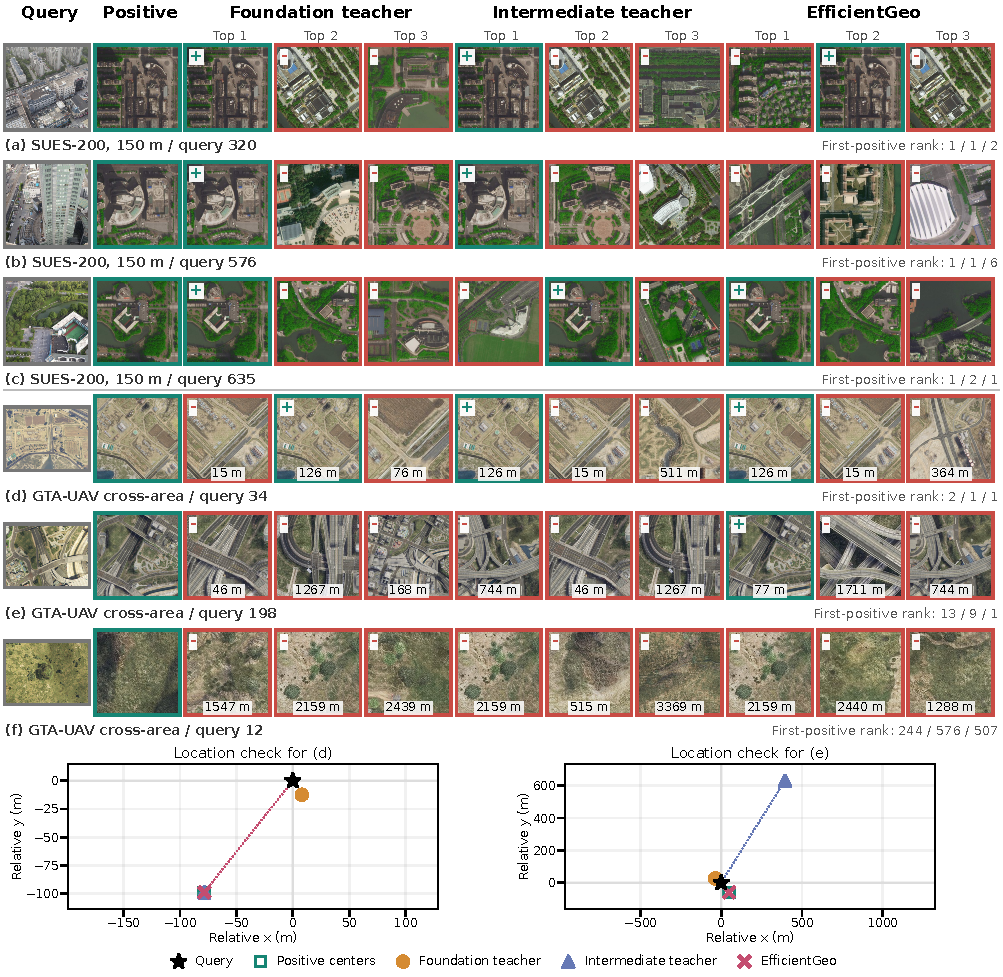
\includegraphics[width=0.88\textwidth]{qualitative_retrieval.pdf}
\caption{Top-3 retrievals on SUES-200 at 150\,m (a--c) and GTA-UAV cross-area (d--f). Green (+) and red ($-$) denote annotated positives and non-positives. First-positive ranks follow the column order: foundation teacher, intermediate teacher, student. The reference is the single SUES-200 positive or the GTA-UAV positive nearest the query. GTA-UAV labels give query-to-tile-center distances; plots show top-1 centers relative to the query. Query IDs are zero-based.}
\label{fig:supp-qualitative}
\endgroup
\end{minipage}\par\addvspace{6pt}
\begin{multicols}{2}
\raggedcolumns
\paragraph{Low-altitude ambiguity and prediction disagreements.}
In (a), the student ranks a similar residential layout above the matching location. In (b), a facade dominates the drone view: both teachers rank the correct location first, but the student ranks it sixth. In (c), the student succeeds where the intermediate teacher ranks the positive second. Across all 150\,m queries, 282 are correct only for the intermediate teacher and 141 only for the student; both succeed on 3,377 and both fail on 200. The cases illustrate layout and facade ambiguities; the counts cover the complete height split.

\paragraph{Exact retrieval versus geographic proximity.}
In (d), the foundation teacher's top-1 is not an annotated positive despite being only 14.8\,m from the query; the other two models retrieve a positive 126.2\,m away. In (e), the student retrieves the correct road junction where both teachers fail. In (f), all three retrieve distant, visually similar vegetation. These cases distinguish exact positive retrieval from geographic proximity.

\end{multicols}
